\comment{Suggestion: present tense, makes sense but might mess up some times H}\\

When referring to the data we will be dealing without throughout this project, it is useful to define quantities clearly to limit the confusion. This was done in~\citep{Project1}, but we will summarise it here.

Letting $\vec{y} \in \mathbb{R}^n$ be a vector containing a series of $n$ measurements with a corresponding to an input matrix $X \in \mathbb{R}^{n\times p}$. The rows $x_i \in \mathbb{R}^p$ of $X$ are the $p$ inputs, or \textit{features}, producing the measurement $y_i$. The feature columns of $X$ are referred to as $\vec{x}_a \in \mathbb{R}^n$. Together these form a dataset $\mathcal{D} = \cclosed{(y_i, x_i)}$. Furthermore, we refer to the parameters of our models collectively by $\vec{\theta}$.

The underlying assumption of our regression is that the measurements $y_i$ are produced from some \textit{exact} function $f(x_i): \mathbb{R}^p \to \mathbb{R}$, with an added stochastic noise $\epsilon$ which follows some unknown distribution. We will further assume that this noise is generated from some normal distribution $\epsilon \distas \normal{0}{\sigma^2}$ with some standard deviation (std) $\sigma$.

In fitting our models to the data, we want to produce predictions $\hat{y} = \hat{f}(x)$ that approximates new measurements $y \sim f(x)$.

\subsection{Gradient Descent Methods}\label[sec]{the:sec:gradient_decent_methods}
    \comment{This section might well be moved to method, it is not too theoretical. -\Carl}\\
    Optimisation of the parameters of the models we will be employing in this project is formulated as minimisation problems, with an associated cost function $C(\vec{\theta})$ to be minimised to find the optimal parameters.
    \subsubsection{Plain Gradient Descent}
        We will compare different variants of GD algorithm, starting first with the plain one. Assume the gradient of the cost function $C(\vec{\theta})$ w.r.t. the parameters $\vec{\theta}$ is well-defined on the entirety of our parameter space, and is calculable either analytically or approximated numerically\footnote{Now this is not always the case, e.g. with $L_1$-penalisation on the parameters.}. The idea is that the fastest direction to move in parameter space to reduce $C(\vec{\theta})$ is to follow the direction of $-\Nablatheta C(\vec{\theta})$. Plain gradient descent implements this idea iteratively, starting from an initial guess $\vec{\theta}_0$, finding the next point by
        \begin{align*}
            \vec{\theta}_{k} = \vec{\theta}_{k-1} - \eta \Nablatheta C(\vec{\theta}_{k-1}),
        \end{align*}
        where $k=1,2,\ldots,N$ for $N$ iterations, and $\eta$ is an introduced hyperparameter called the learning rate.

    \subsubsection{Adding Momentum}
        The simple GD can be fleshed out by giving the algorithm a sense of inertia, helping it continue to move in a certain direction. This combats tendency to oscillate around saddle points, for instance. It starts as earlier, but with the additional initialisation $\vec{p}_0 = 0$, finding $\vec{\theta}_k$ iteratively by 
        \begin{subequations}
            \begin{align}
                \vec{p}_{k} &= \gamma \vec{p}_{k-1} + \eta \Nablatheta C(\vec{\theta}_{k-1}), \\
                \vec{\theta}_k &= \vec{\theta}_{k-1} - \vec{p}_k,
            \end{align}
        \end{subequations}
        where $\gamma$ is a new hyperparameter characterising the memory of earlier gradients.

    \subsubsection{Stochastic Gradient Descent} 
        Stochastic Gradient Descent (SGD) is based on functions to minimise that are on the form $C(\vec{\theta}) = \sum_{i \in A} c_i(\vec{\theta}) + c_0(\vec{\theta})$ for $A=\cclosed{1,2,\ldots,n}$. This is often the case, as in MSE-scores, where a cost is associated with every observation $y_i$ separately. The idea of SGD is to avoid computing the gradient of the whole of $C$, but rather split it into mini-batches $C_k(\vec{\theta}) = \sum_{i\in A_k} c_i(\vec{\theta}) + c_0(\vec{\theta})$ for some subset $A_k \subseteq A$, and compute the gradient only on one of these smaller batches. This helps solve two problems: First, it makes the computational cost of calculating the gradient smaller, as we no longer compute the full one, and second, it adds a degree of stochasticity to the movement in parameter space since we no longer will follow the `true' gradient, which prevents getting stuck in local minima.

        SGD is done in so-called epochs, where we divide the full set $A$ into equally sized batches $A_k$, and do one GD iteration on every batch once. After this, $A$ is reshuffled and new mini-batches are drawn.

    \subsubsection{Improving Convergence Rate}
        As stochasticity is added to the algorithm, the rate of convergence does slow down. As such, it would be nice to add algorithms that can adapt the learning rate $\eta$ in such a way as to increase the rate of convergence. The AdaGrad algorithm does this with the idea to use different learning rates along different directions in parameter space; i.e. use larger learning rates in flat directions, while keeping it small in steep directions. This is done by keeping a running sum $G_k$ of the outer product of the gradients $\vec{g}_k$ at the points $\vec{\theta}_k$, and use this to adapt the learning rate.
        \comment{I don't know whether to include the update rules in the \LaTeX-document, or maybe move them to method, or whatever. -\Carl}
        \begin{subequations}
            \begin{align}
                \vec{g}_k &= \Nablatheta C_k(\vec{\theta}_{k-1}) \\
                G_k &= G_{k-1} + \vec{g}_j \otimes \vec{g}_j \\
                \vec{\theta}_k &= \vec{\theta}_{k-1} - \eta G_k^{-\sfrac{1}{2}} \vec{g}_k
            \end{align}
            where $\vec{v} \otimes \vec{u}$ denotes the outer product of two vectors $\vec{v}, \vec{u}$, and a matrix $m = M^{-1/2}$ is understood to the matrix satisfying $m^2 = M^{-1}$. Inverting and finding the root of $G_k$ comes at a computational cost, so we will employ the much cheaper version where we update \comment{Discussion note: mention uncorrelated features bettering this approximation, perhaps. -\Carl}
            \begin{align}
                \vec{\theta}_{k} = \vec{\theta}_{k-1} - \frac{\eta}{\sqrt{\diag(G_k)}+\epsilon} \circ \vec{g}_k,
            \end{align}
        \end{subequations}
        where the arithmetic operations are understood to be element-by-element and $\vec{v}\circ \vec{u}$ represents the element-wise multiplication of two vectors $\vec{v}, \vec{u}$, and $\epsilon$ is a small number to avoid zero-division.
        
        The AdaGrad algorithm serves to tune the learning rate, and can be applied to gradient descent with momentum too. This gives the update rule
        \begin{subequations}
            \begin{align}
                \vec{g}_k &= \Nablatheta C_k(\vec{\theta}_{k-1}) \\
                \vec{p}_k &= \gamma \vec{p}_{k-1} + \eta \vec{g} \\
                G_k &= G_{k-1} + \vec{g}_j \otimes \vec{g}_j \\
                \vec{\theta}_k &= \vec{\theta}_{k-1} - \frac{\eta}{\sqrt{\diag(G_k)}+\epsilon} \circ \vec{p}_k
            \end{align}
        \end{subequations}

        Another way to adapt the learning rate to the parameter space `terrain' is found in the Root Mean Square Propagation (RMSprop) algorithm. Here we approximate a running average of the second moment of the gradient $\vec{s} = \expval(\vec{g} \circ \vec{g})$, then use this to scale the learning rate appropriately.
        \begin{subequations}
            \begin{align}
                \vec{g}_k &= \Nablatheta C_k(\vec{\theta}_{k-1}) \\
                \vec{s}_k &= \beta \vec{s}_{k-1} + (1-\beta) \vec{g}_k \circ \vec{g}_k \\
                \vec{\theta}_k &= \vec{\theta}_{k-1} - \frac{\eta}{\sqrt{\vec{s}_k}+\epsilon} \circ \vec{g}_k
            \end{align}
        \end{subequations}
        where again $\epsilon$ is a small number to avoid zero-division, and the arithmetic operations are understood to be element-wise. Here $\beta \in [0,1]$ is a new hyperparameter parametrising the rate at which previous gradients should inform the current average of the second moment.

        Finally, an algorithm which aims to combine RMSprop with momentum is Adam. Here we also keep a running average of $\vec{m} = \expval(\vec{g})$, i.e. the first moment of the gradient. Moreover, bias-corrected values are used in lieu of the `bare' estimates of the first and second moments, here denoted with hats. This ensures that a bias for low values of $\vec{m}_k, \vec{s}_k$ in early iterations with high $\beta$-values is avoided.
        \begin{subequations}
            \begin{align}
                \vec{g}_k &= \Nablatheta C_k(\vec{\theta}_{k-1}) \\
                \vec{m}_k &= \beta_1 \vec{m}_{k-1} + (1-\beta_1) \vec{g}_k \\
                \vec{s}_k &= \beta_2 \vec{s}_{k-1} + (1-\beta_2) \vec{g}_k \circ \vec{g}_k \\
                \vec{\hat{m}}_k &= \frac{\vec{m}_k}{1-\beta_1^k} \\
                \vec{\hat{s}}_k &= \frac{\vec{s}_k}{1-\beta_2^k} \\
                \vec{\theta}_k &= \vec{\theta}_{k-1} - \frac{\eta}{\sqrt{\vec{\hat{s}}_k}+\epsilon} \circ \vec{\hat{m}}_k
            \end{align}
        \end{subequations}


    \subsection{Neural Networks}
        Artificial neural networks (ANN) are biologically inspired machine learning algorithms which can improve performance as they are exposed to data and without being programmed with any task-specific rules. In this project fully connected Feed-Forward Neural Networks (FFNN) will be implemented. 
        \subsubsection{Structure}
            First a non-mathematical, intuitive introduction. 
            An ANN consists of an input layer and an output layer. Often the network will also have layers between the input and output, called \textit{hidden layers}. In that case the neural network is often referred to as deep. Each layer contains \textit{nodes} which are supposed to represent the neurons in a biological neural network, or rather their activation. In a fully connected neural network, all nodes in one layer are connected to all the nodes in the previous as well as the next layer. These connections, which represent the synapses, are referred to as \textit{weights}, and the sizes of the weights are the synaptic strength. Each node also have an activation \textit{bias} which says something about how easily activated that specific neuron/node is. See \cref{the:fig:Illustration_NN} for an illustration of a simple artificial neural network. 
            \begin{figure} [ht]
                \centering
                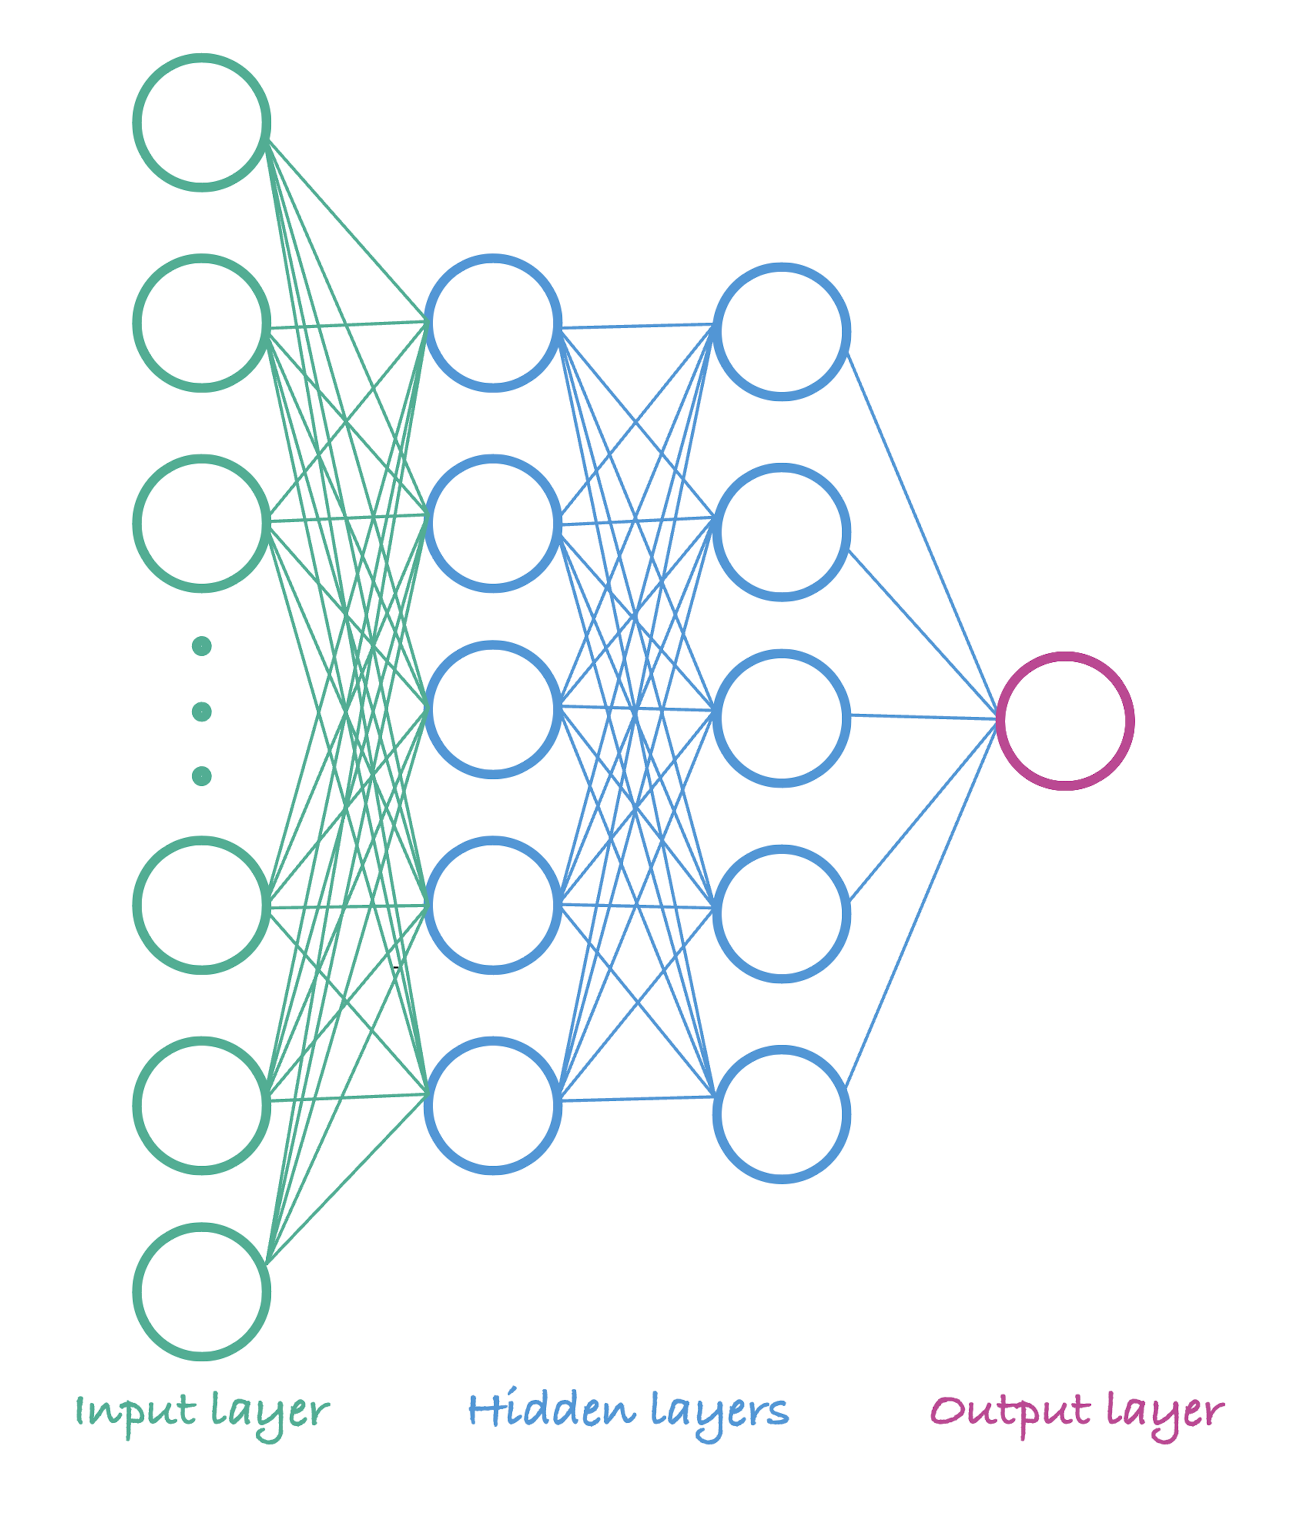
\includegraphics[width=.85\linewidth]{figs/Illustration_NN.png}
                \caption{Illustration of a simple deep neural network with an input layer, two hidden layers, and an output layer. The circles are the nodes and the lines between are the weights.}
                \label[fig]{the:fig:Illustration_NN}
            \end{figure}
            
            The nodes, weights and biases are all essentially just numbers, but following an algorithm for combining these numbers creates an ANN. 

        \subsubsection{Feed Forward}
            \begin{figure} [ht]
                \centering
                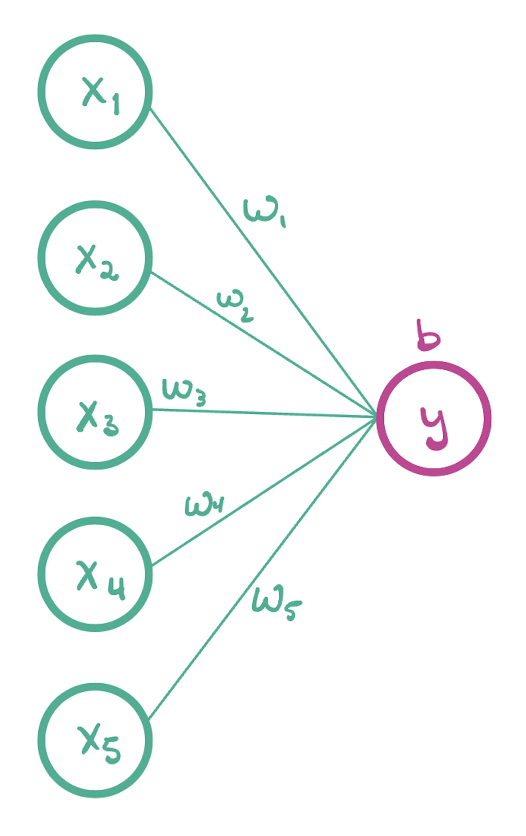
\includegraphics[width=.4\linewidth]{figs/Illustration_simple.png}
                \caption{Illustration of a simple neural network with an input layer, and an output layer consisting of one node.}
                \label[fig]{the:fig:simple_NN}
            \end{figure}
            The simplest of neural networks is the \textit{Feed Forward Neural Network(FFNN)} which, as its name implies, feeds activation from the input layer and forward through the network, eventually ending up in the output layer. Given a NN with only an input layer, and an output layer consisting of one node (see \cref{the:fig:simple_NN}), the output $\hat{y}$ is then  
            \begin{equation}
                \hat{y}=f\left(\sum_{i=1}^n w_i x_i+b\right)= f(z)
            \label[eq]{the:eq:output}
            \end{equation} 
            where $x_i$ constitutes the input, $w_i$ are the weights corresponding to each input variable, and $b$ the bias of the output node. We define $z$ as the sum over all the weighted inputs with bias added; $z=\pclosed{\Sigma_{i=1}^n w_ix_i + b}$. $f$ is called the \textit{activation function} and depends on the analysis being executed; e.g. regression, classification, etc. Each node in a network has a corresponding activation function which defines the possible outputs of that node. The activation function closest to replicating the behaviour of a biological neuron is the Heaviside function which yields either $0$ or $1$; firing or not firing. However, there are in some cases advantages of abandoning this biological model. Some other, and currently more used activation functions are: identity, sigmoid, ReLU, tanh, and leaky ReLU some of which are plotted in \cref{the:fig:introducing_acts}. 
            \begin{figure} [ht]
                \centering
                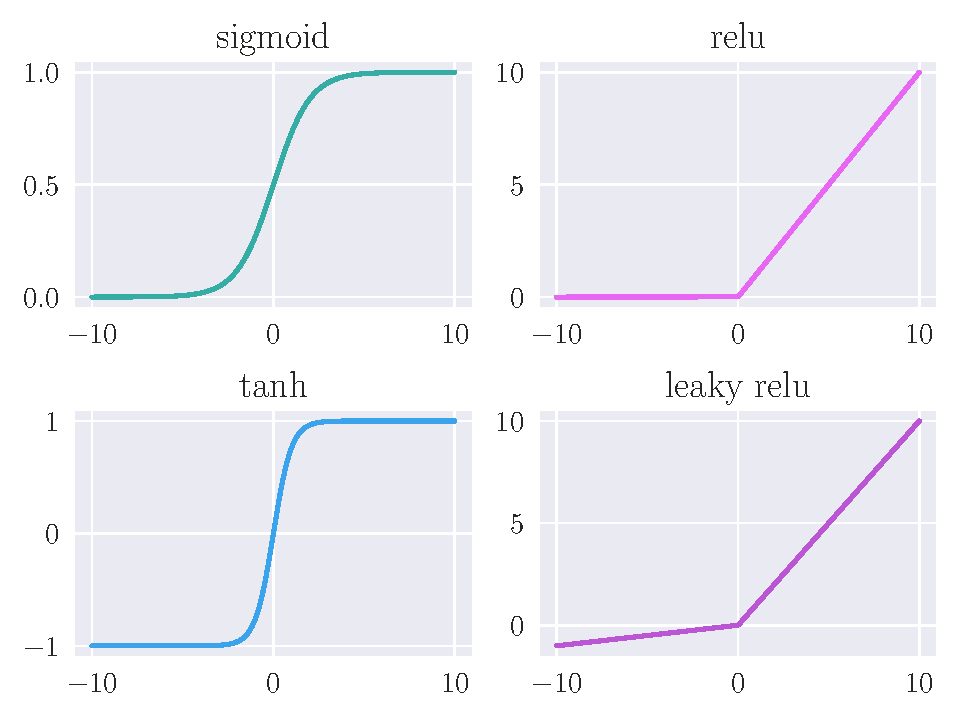
\includegraphics[width=\linewidth]{figs/introducing_acts.pdf}
                \caption{Plots of some commonly used activation functions.}
                \label[fig]{the:fig:introducing_acts}
            \end{figure}
            
            In the output layer the activation function constitutes what analysis the network does. E.g. a form of binary classification can be done by implementing the sigmoid activation function in the output layer, and for regression problems the identity function, $f(x)=x$, is implemented.
            It is normal that all the nodes in a layer have the same activation function $f$.    
            \comment{See more on activation functions in appendix ref} 

            If we were to have a more complex neural network than the one from \cref{the:fig:simple_NN}, now also including hidden layers, $\hat{y}$ (ref \cref{the:eq:output}) would be a node in the hidden layer after the input. Each node in the network would have its own activation bias and would be connected with the input, or activation from the previous layer, through independent weights. \cref{the:eq:node_activation} shows the calculated activation of a specific node $i$ in layer $l$ of the network.
            \begin{equation}
                a^l_i = f^l \pclosed{\sum_{j=1}^{N_{l-1}} w_{ij}^l a_j^{l-1} + b^l} = f^l(z^l_i)
            \label[eq]{the:eq:node_activation}
            \end{equation}  
            \begin{equation}
                z^l_i = \sum_{j=1}^{N_{l-1}} w_{ij}^l a_j^{l-1} + b_i^l
            \end{equation}
            This can be written in a more compact form like in \cref{the:eq:node_activation_compact}.
            \begin{equation}
                \vec{z}^l = \pclosed{W^l}^T\vec{a}^{l-1} + \vec{b}^l
                \label[eq]{the:eq:node_activation_compact}
            \end{equation}
            The activations of the first layer go into calculating the activations of the next layer, which again go into the next, and then the next, until the activations of the output layer, $\vec{a}^L \equiv \hat{y}$, are found. 



        \subsubsection{Backpropagation}
            The essence of neural networks as machine learning is \textit{training}. This means getting the network to adjust its parameters to better fit the data. A common algorithm used to do this is the \textit{Backpropagation algorithm}. A feed forward calculation of the network yields an output which can be compared with the true data output through a cost function. The goal is to minimise the cost. The only changes the network can do to get a different output, is to adjust its weights and biases. Backpropagation is a method of finding the gradients of the cost function with respect to these parameters. The gradients are calculated through the chain rule and for one layer at the time, starting at the last layer and propagating backwards through the network, hence the name Backpropagation. When these are found one can apply a gradient descent method for finding the parameters yielding the lowest cost and implementing them in the network. After a feed forward pass with the new parameters, the process of backpropagation, gradient descent, and updating can be repeated. This is a way of training the network.     
            
            Mathematically, finding the gradients of the individual weights, $w_{ij}$, and biases, $b_i$, for the last layer $L$ can be done as in \cref{the:eq:bp_w_b_delta}.
            \begin{subequations}
                \label[eq]{the:eq:bp_w_b_delta}
                \begin{align}
                    \pdv{C}{b_i^L} &= \pdv{C}{z_i^L} \pdv{z_i^L}{b_i^L} = \pdv{C}{z_i^L} \equiv \delta_i^L 
                \label[eq]{the:eq:bp_w}
                \end{align}                
                \begin{align}
                    \pdv{C}{w_{ij}^L} = \pdv{C}{z_i^L}\pdv{z_i^L}{w_{ij}^L} = \delta_i^L a_j^{L-1}
                \label[eq]{the:eq:bp_b}
                \end{align}
                \begin{align}
                    \delta_i^L = \pdv{C}{z_i^L} = \pdv{C}{a_i^L}\pdv{a_i^L}{z_i^L} = \pdv{C}{a_i^L} f'(z_i^L)
                \label[eq]{the:eq:bp_delta} 
                \end{align}
            \end{subequations}
            All of these equations are independent of the cost function implemented and enables the use of automatic differentiation through tools like e.g. \verb|Autograd|. It is also possible to calculate all of these sizes analytically, but that yields less flexibility in the neural network. By the same approach, the gradients for the layers $l = L-1, L-2,...,1$ can be found: 
            \begin{subequations}
                \begin{align}
                    \delta_i^l = \pdv{C}{z_i^l} = \sum_k \pdv{C}{z_k^{l+1}} \pdv{z_k^{l+1}}{z_i^l} 
                    = \sum_k \delta_k^{l+1} \pdv{z_k^{l+1}}{z_i^l}
                \end{align}
                \begin{align}
                    z_k^{l+1} = \sum_{j=1}^{N_l} w_{ki}^{l+1} a_i^l + b_k^{l+1}
                \end{align}
                \begin{align}
                    \delta_i^l = \sum_k \delta_k^{l+1} w_{ki}^{l+1} f'(z_i^l)
                \end{align}
                \begin{align}
                    \pdv{C}{b_i^L} = \delta_i^l \quad \wedge \quad 
                    \pdv{C}{w_{ij}^L} = \delta_i^l a_j^{l-1}                
                \end{align}
            \end{subequations}
            \comment{Maybe remove the last two eqs?}
            Having found the gradients of the parameters for all the layers, gradient descent can be implemented. 

    \subsubsection{Universal Approximation Theorem}
        A lot of the promise of NNs comes from the fact that they are \textit{universal approximators}. It has been shown (\citep{HornikEtAl89}) that a neural network with only a single hidden layer can approximate arbitrarily well any function $f(x): \mathbb{R}^n \to \mathbb{R}$ for any (positive) integer $n$. This requires the activation function of the hidden layer fulfil certain requirements: Namely being a non-constant, bounded and monotonically increasing, continuous function~\citep{MortenUAT}.



\subsection{Classification}
    Instead of predicting targets in a continuous domain ($y_i \in \mathbb{R}$), we aimed to put the target $y_i$ in a specific class ($y_i \in \mathcal{Q}$), where $\mathcal{Q}$ is the set of possible outcomes. This is named \textit{classification} \comment{Is this perhaps a bit confusing nomenclature? -\Carl}, where in the following we will only consider binary cases. This means we will try to classify mutually exclusive properties, that is either we have the outcome $O$ or not the outcome $O$ ($\mathcal{Q} = \{O, \neg O\}$). We will label these as $O = 1$ and $\neg O = 0$.

    Two different methods for classification will be introduced here. Firstly we will look at \textit{logistic regression}, maybe the most common method in the domain of classification. In addition, under some restrictions, our neural network can be used for classification problems. Both of these models have an output $p(x_i)$ on the domain $[0,1]$, which we will interpret as the probability of the outcome $y_i = 1$. We will classify the data point $x_i$ as $\hat{y}_i = 1$ if $p(x_i) > \tau$ and $\hat{y}_i = 0$ if $p(x_i) < \tau$, where $\tau$ is the \textit{threshold}, a priori set to $\tau = 0.5$. 

    \subsubsection{Logistic Regression}
        For comparison with our neural network we introduce maybe the most common classification method there is, \textit{logistic regression}. One might be confused by inclusion of the word \textit{regression} in the name of a classification method. This comes from performing a fit to the \textit{log-odds} using a function linear in the input variables:
        \begin{align*}
            \log(\frac{p(x_i)}{1-p(x_i)}) = x_i^T \vec{\theta},
        \end{align*}
        where we have defined $p(x_i) \equiv p(y_i = 1 | x_i, \vec{\theta})$, the probability that we guess $\hat{y}_i = 1$ given a data point $x_i$ and parameters $\vec{\theta}$. Solving the above expression for $p(x_i)$ yields the Sigmoid function from \cref{app:activation_functions} evaluated in $x_i^T \vec{\theta}$. \comment{I might be tripping, but I can't see where the sign in the exponent comes from. -\Carl}
        
        \begin{align*}
            p(x_i) = \sigma(x_i^T \vec{\theta}) = \frac{1}{1+\exp{-x_i^T\vec{\theta}}}
        \end{align*}
        Following the approach from \citep{Project1}, we have the likelihood for a Binomial distribution:      

        \begin{align*}
            P(\vec{y}|X,\vec{\vec{\theta}}) = \prod_{i = 1}^{n} \sigma(X_{i*}\vec{\theta})^{y_i}[1-\sigma(X_{i*}\vec{\theta})]^{1 - y_i},
        \end{align*}
        where a sum over $a$ is implied. The cost function then follows from taking logarithm of the likelihood, presented with an overall negative sign giving a minimisation problem of the parameters $\vec{\theta}$. In the literature this is often called the \textit{Binary Cross Entropy} (BCE) cost function \citep{BCE}.  

        \begin{align}
            \msub{C}{BCE}(\vec{\theta}) =& - \frac{1}{n} \log P(\vec{y}|X,\vec{\vec{\theta}}) \nonumber \\ \nonumber
            =& - \frac{1}{n} \sum_{i = 1}^{n} \Big\{ y_i \log[\sigma(X_{i*}\vec{\theta})] \\
            &+ (1 - y_i)\log[1-\sigma(X_{i*}\vec{\theta})] \Big\}
            \label[eq]{the:eq:logreg_cost_function}
        \end{align}
        Taking the derivative wrt. to a parameter $\theta_b$ recalling the derivative of the Sigmoid function from \cref{app:activation_functions} we find:

        \begin{align} \nonumber
            \pdv{\theta_b} \msub{C}{BCE} =& - \frac{1}{n} \sum_{i = 1}^{n} \Big\{ y_i \bclosed{1-\sigma(X_{i*}\vec{\theta})}X_{ib} \\ \nonumber
            &- (1-y_i)\sigma(X_{i*}\vec{\theta})X_{ib}  \Big\} \\
            =& \frac{1}{n}\sum_{i=1}^n \bclosed{\sigma(X_{i*}\vec{\theta}) - y_i}X_{ib}
        \end{align}
        Finally, with $p(x_i) = \sigma(X_{i*}\vec{\theta})$, we can express the gradient of the BCE cost function in vector notation.
        \begin{align}
            \nabla_{\vec{\theta}} \msub{C}{BCE}(\vec{\theta}) = \frac{1}{n}X^T (\vec{p} - \vec{y}) 
            \label[eq]{the:eq:logreg_gradient}
        \end{align}


    \subsubsection{Neural Network Approach}
        Something Something since we want to interpret output as probability we must choose Sigmoid. Hidden activation functions can be whatever. 